%%%%%%%%%%%%%%%%%%%%%%%%%%%%%%%%%%%%%%%%%%%%%%%%%%%%%%%%%%%%%%%%%%%%%%%%%%%%%%%%
%2345678901234567890123456789012345678901234567890123456789012345678901234567890
%        1         2         3         4         5         6         7         8

\documentclass[letterpaper, 10 pt, conference]{ieeeconf}  % Comment this line out if you need a4paper
\usepackage[utf8]{inputenc}
\usepackage{graphicx}
\usepackage{amsmath}
\usepackage{hyperref}
\usepackage{cleveref}
\usepackage{amssymb}
\usepackage[table]{xcolor}% http://ctan.org/pkg/xcolor
\usepackage{xcolor}
\usepackage{epsfig}
\let\labelindent\relax
\usepackage{enumitem}
\usepackage{pgf,tikz}
\usetikzlibrary{decorations.pathreplacing,calligraphy}
\usepackage{makecell}
\usepackage{mdframed}% http://ctan.org/pkg/mdframed
%\usepackage{geometry}

%\documentclass[a4paper, 10pt, conference]{ieeeconf}      % Use this line for a4 paper

\IEEEoverridecommandlockouts                              % This command is only needed if 
% you want to use the \thanks command

\overrideIEEEmargins                                      % Needed to meet printer requirements.

%In case you encounter the following error:
%Error 1010 The PDF file may be corrupt (unable to open PDF file) OR
%Error 1000 An error occurred while parsing a contents stream. Unable to analyze the PDF file.
%This is a known problem with pdfLaTeX conversion filter. The file cannot be opened with acrobat reader
%Please use one of the alternatives below to circumvent this error by uncommenting one or the other
%\pdfobjcompresslevel=0
%\pdfminorversion=4

% See the \addtolength command later in the file to balance the column lengths
% on the last page of the document

% The following packages can be found on http:\\www.ctan.org
%\usepackage{graphics} % for pdf, bitmapped graphics files
%\usepackage{epsfig} % for postscript graphics files
%\usepackage{mathptmx} % assumes new font selection scheme installed
%\usepackage{times} % assumes new font selection scheme installed
%\usepackage{amsmath} % assumes amsmath package installed
%\usepackage{amssymb}  % assumes amsmath package installed

%\title{\LARGE \bf
%	JAEGO : Attention Sharing in Sensory Egocentric Spheres
%}
%\title{\LARGE \bf
%	From Egocentric Sensory Sphere to Joint Attention and Back 
%}
\title{\LARGE \bf
	JA-EGO : The Egocentric Dimension of Joint Attention in HRI
}


\author{Hendry F. Chame$^{1}$ and Rachid Alami$^{2}$% <-this % stops a space
	%\thanks{*This work was not supported by any organization}% <-this % stops a space
	\thanks{$^{1}$Team NeuroRhythms at LORIA-CNRS, Campus Scientifique, 615 Rue du Jardin-Botanique, 54506 Vand\oe uvre-l\`es-Nancy, France.
		{\tt\small hendry.ferreira-chame@loria.fr}}%
	\thanks{$^{2}$Team Robotics and InteractionS (RIS) at LAAS-CNRS, Universit\'e de Toulouse, CNRS, Toulouse, France
		{\tt\small rachid.alami@laas.fr}}%
}


\begin{document}
		
	
	\maketitle
	\thispagestyle{empty}
	\pagestyle{empty}
	
	
	%%%%%%%%%%%%%%%%%%%%%%%%%%%%%%%%%%%%%%%%%%%%%%%%%%%%%%%%%%%%%%%%%%%%%%%%%%%%%%%%
	\begin{abstract}
		
		\small \bf Despite important progress in recent years, there is a long way to go for including social robots in our environments, capable of adaptation, interaction and communication. Our research is concerned with the study of social cognition in HRI, in particular with communication skills relying on joint attention (JA) and knowledge sharing. Since JA involves low-level cognitive skills, we take into account the implications addressed by Moravec's Paradox and focus on the aspect of knowledge representation. By embracing embodiment and 4E cognition principles, we investigate the notion of egocentric localization and propose a neural network representation suited for joint attention research named JA-EGO. Inspired by \textit{dynamic fields theory}, the model consists in a dynamical system representation which fuses information from immediate sensation and provides the means for attention selection and working memory under the influence of top-down and bottom-up modulation processes of attention in HRI. We firstly studied the attention selection model in simulations application scenarios. We then conducted a real experiment with the robot Pepper considering egocentric sources of information and basic proxemics. Results showed that JA-EGO is a convenient representation for HRI situations allowing the human and the robot to share attention and knowledge about objects in the environment. 
		
		%\small \bf Despite important progress in recent years robots are still far behind from exhibiting the sophistication of cognitive skills observed in human beings. Our research is concerned with the study of social cognition in HRI, in particular with the concept of joint attention (JA) and knowledge sharing. Given the fact that JA involves low-level cognitive skills, we take into account the implications addressed by Moravec's Paradox and consider the aspect of knowledge representation as crucial for HRI. Hence, our work departs from views of JA based on cognitivist philosophy and embraces embodiment and 4E cognition principles, as a source of inspiration for proposing adaptable and efficient models of interaction which do not depend extensively on environmental modeling and variable control. Within this direction, in this work we explore the notion of egocentric spherical localization and propose a neural network representation of the human and the robot attention state named JA-EGO. Inspired by dynamic fields theory, the model consists in a dynamical system representation provided with information from low-level sensory acquisitions representing cognitive skills such as attention selection from immediate sensation. We tested the model firstly in simulations for exploring some application scenarios. We then conducted a real experiment with the robot Pepper considering local (egocentric) sources of information and basic proxemics. Results showed that JA-EGO is a convenient representation for HRI situations allowing the human and the robot to share attention and knowledge about objects in the environment. 
		
		
		
		
		%In everyday life we frequently run into face-to-face interactions where we quickly share attention and communicate about objects with others. In such situations, we can talk about things in the environment even when seeing for the first time. As addressed in Moravec's Paradox, for human-robot interaction research, the scenario is not as simple as for human interaction. However, progress has been achieved when departing from cognitivist philosophy and embracing embodiment and 4E cognition research, as a source of inspiration for designing light and efficient models of interaction. This work goes in this direction and proposes a neural network for ego-spheric sensory fusion named JA-EGO relying mostly on immediate sensation and low level cognitive skills such as working memory, so a robot is able to share attention with the human based on local (egocentric) sources of information and basic proxemics. The advantage of our approach is that, by exploiting embodiment, a very efficient and intuitive communication system can result, which is adaptable to everyday situations not requiring the agent to process extensive information about the environment. In order to assess our hypothesis, we performed studies in simulation and a real interaction with the robot Pepper in a joint attention task. Results showed the robot is able to correctly focus on objects of interest in the environment when interacting with the human.
		
		%\small \bf In everyday life we frequently run into face-to-face interactions where we quickly share attention and communicate about objects with others, be it for providing guidance to someone or commenting or some unusual thing or event, to name a few examples. In such situations, we don’t think too much about it, although we may not necessarily know where we are, we can talk about things in the environment even when seeing for the first time. As addressed in Moravec's Paradox, for human-robot interaction research, the scenario is not as simple as for human interaction. However, progress has been achieved when departing from cognitivist philosophy and embracing embodiment and 4E cognition research, as a source of inspiration for designing light and efficient models of interaction. This work goes in this direction and proposes a neural network for ego-spheric sensory fusion named JA-EGO relying mostly on immediate sensation and low level cognitive skills such as working memory, so a robot is able to share attention with the human based on local (egocentric) sources of information and basic proxemics. The advantage of our approach is that, by exploiting embodiment, a very efficient and intuitive communication system can result, which is adaptable to everyday situations not requiring the agent to process extensive information about the environment. In order to assess our hypothesis, we performed studies in simulation and a real interaction with the robot Pepper in a joint attention task. Results showed the robot is able to correctly focus on objects of interest in the environment when interacting with the human.   
		
	\end{abstract}
	
	
	%%%%%%%%%%%%%%%%%%%%%%%%%%%%%%%%%%%%%%%%%%%%%%%%%%%%%%%%%%%%%%%%%%%%%%%%%%%%%%%%
	\section{INTRODUCTION}
	
	According to Moravec's paradox, although machines can perform tasks at adults' level of reasoning and intelligence (like playing checkers), they have tremendous difficulty with sensory-motor or social skills, as demonstrated by a one-year-old child. Behind this paradox remains the question in artificial intelligence research of what sort of knowledge representation would be suitable for allowing a machine to accomplish cognitive tasks, which has important philosophical implications. Recent research has contrasted from one side the Cartesian (traditional) view of social cognition as a process confined to the brain, to the notion of an \textit{embodied}, \textit{embedded}, \textit{enacted} and \textit{extended} process, unfolding between the brain, the body and environment in interaction; a perspective known as \textit{4E cognition} \cite{Newen2018}.      
	
	From the perspective of 4E cognition research, we believe that for social robots to leave the lab and adapt to human environments, it is crucial to provide them with forms of behavior regulation which take into account the dynamics of human low-level social skill processes such as the capacity of engaging in \textit{joint attention} (JA), and the possibility of such processes be modulated in direct interaction. Moreover, we study JA as a multi-dimensional construct involving cognitive skills so constituting forms of social attention at distinct levels of interaction and knowledge sharing \cite{siposova2019}. 
	
	As a continuation of previous research in which we proposed a model for tracking JA in HRI within a topology-based representation constituting a \textit{scale of jointness} \cite{chame2023top}, in this work we investigate the more fundamental aspect of attention selection and how such mechanism could allow the emergence of JA in human-robot interaction from top-down and bottom-up modulation processes. For this, we suppose unconstrained situations where agents can become interested in objects on the environment and eventually share attention and knowledge about it (e.g. situations like asking someone for direction or commenting about salient stimulus like a noise or an object). 
	
	From the considerations above, we propose the model named JA-EGO for tracking the attention focus of agents as represented from egocentric perspective, and resulting from acquisitions from robot's on-board sensory of agents body posture and local stimulus. For this, we model the evolution of attention selection as a dynamical system process represented by a neural network inspired on \textit{dynamic neural fields} theory \cite{amari1977}, which tracks egocentric focus of attention from spherical localization references. 
	  
	  
	This document is organized as follows: Section \ref{sec:previous} discusses previous works and contextualizes our contribution according to limitations in state of the art research. Section \ref{sec:model} presents the mathematical definition of the model and discusses theoretical assumptions behind it. Section \ref{sec:methodology} describes the methodology of the work, consisting in a preliminary study conducted in simulation for evaluating attention tracking based on the selection process, followed by an experiment with the robot Pepper considering a joint attention interaction situation based on egocentric sources of information and basic proxemics about objects in the environment. Section \ref{sec:results} reports the study’s results, and Section \ref{sec:conclusions} presents conclusions and future perspectives.
	  
%	For this, an egocentric perspective for localization is adopted where the robot is able to represent the dynamics of its own focus of attention in an sensory ego-spherical representation as well as tracking others' focus of attention. 
	
	
	\section{PREVIOUS WORK}
	\label{sec:previous}
	
	%Biological studies have pointed out to the existence of biological mechanisms to support essential cognitive functions such as attention, short-term memory, spatio-temporal sensory-motor coordination, and locomotion, among others.

	Some works in the field of robotics have achieved impressive results by exploring attention saliency in sensory egocentric representations (e.g. for bottom-up \cite{ruesch2008} and top-down \cite{bodiroza2011} mechanisms). Most of these works have considered a sort of environment exploration task, so the robot can focus on learning new things based on novelty. Fewer research have studied joint attention tasks (e.g. \cite{bodiroza2011}) inspired on psychological theories of attention. Overall, the representation proposed has neglected bio-inspiration on neural systems, consisting mostly in storage arrays for data indexed by spherical tessellation mapping (see \cite{peters2009sensory}). As a result, the dynamics of pre-attentive processing has not being modeled as a process unfolding in the same space where attention selection is done. We believe that this is an important limitation, when considering the possibility of investigating compositionality in joint attention as a descending (top-down) generative process combined with an ascending (bottom-up) saliency process, susceptible of study as a dynamical system.   
	
	Another limitation of previous research is considering the robot as the only one in interaction given with embodied ego-sensory mapping representations, so data coming from the human is mostly represented in the robot ego-sensory sphere. In our opinion, this would be a too much egocentric view of joint action in HRI. Thus, the robot should be able to represent its own world while accepting the egocentric view of others and being able to handle such body correspondences dynamically. 
	 
	From our perspective, different works have constituted previous steps in the direction of proposing our current study which is worth mentioning. The work by \cite{chame2016} has proposed a sensory ego-cylindrical information fusion mechanism for egocentric localization allowing the robot to autonomous position with respect to object in the environment based on embodied representations. Concerning joint attention modeling, the model TOP-JAM \cite{chame2023top} was proposed for interaction situations mediated by objects where allocentric references for addressing the task would make sense (e.g. sharing attention around a table, participating in an assembly collaboration task, to name a few) considering an extended range of knowledge and attention sharing (i.e. individual, monitoring, common, and sharing \cite{siposova2019}). 
	 
	
	% 
	
	
	%More importantly, attention clues from the human are not processed in the same representation space
	
	%attention processes dynamics has not been 
	
	%the body posture of the human has not being considered as an source of information for the robot attention process. Moreover, the sensory ego-sphere has been proposed as a computational data structure which does not represents directly the focus of attention of participants, neglecting thus the dynamics of interaction, consisting mostly in a data storage repository indexed by tessellation spherical mapping (see \cite{peters2009sensory}). 
	
	
	
	
	%\cite{ruesch2008}
	
	%The problem of placement of the egocentric localization reference is not trivial and would greatly depend on the task at hand.   
	
	%The origin of the ego-cylinder can be fixed to different parts of the body. There is no agreement in the literature on the placement for this structure.
	
	
	 %... in the field of cognitive robotics, the work by \cite{peters2009sensory} has proposed a data structure in the form of a sensory ego-sphere located at the robot base frame as a mediating interface between sensors and cognitive processes. 
	 
	%The work by \cite{chame2016} has proposed a sensory ego-cylindrical information fusion mechanism for egocentric localization allowing the robot to autonomous position with respect to object in the environment based on embodied representations. 
	
	\begin{figure}[h!]
		\begin{center}
		\begin{tikzpicture}
		\node [] at (0,0){
			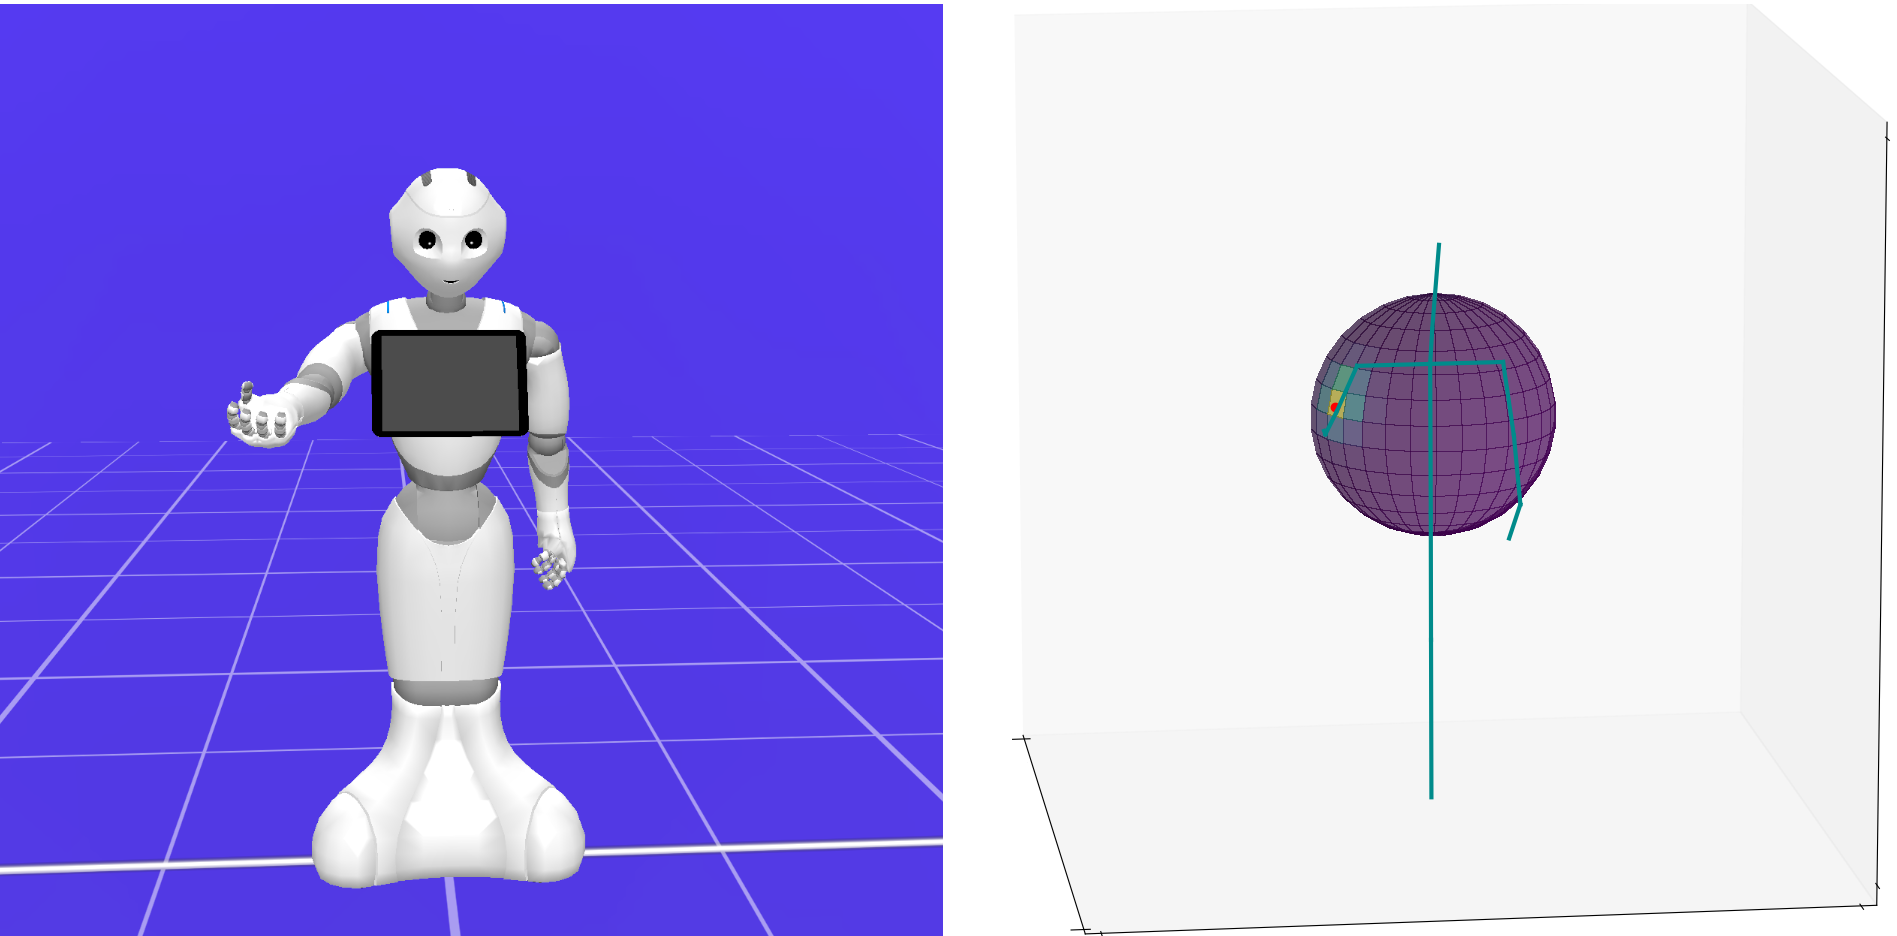
\includegraphics[scale=0.5,keepaspectratio]{fig/robot_pointing.png}};
		\node at (0.0,2.4) [color=black] {\small \textbf{The robot sensory ego-sphere}};
		\end{tikzpicture}
		\caption{Left: the robot is pointing to a location in the space. Right: the attention state of the robot is shown as the activation of the neural network representing the sensory ego-sphere, as stimulated by the intersection of the forearm direction with by the sensory ego-sphere.}
		\label{fig:robot_pointing}
		\end{center}
	\end{figure}

	
	\section{THE MATHEMATICAL MODEL}
	
	\label{sec:model}
	Let a ego-sphere representation of sensory information be modeled by the following neural network architecture \cite{amari1977}.
	
		\begin{figure}[h!]
		\begin{center}
			\begin{tikzpicture}
			\node [] at (0,0){
				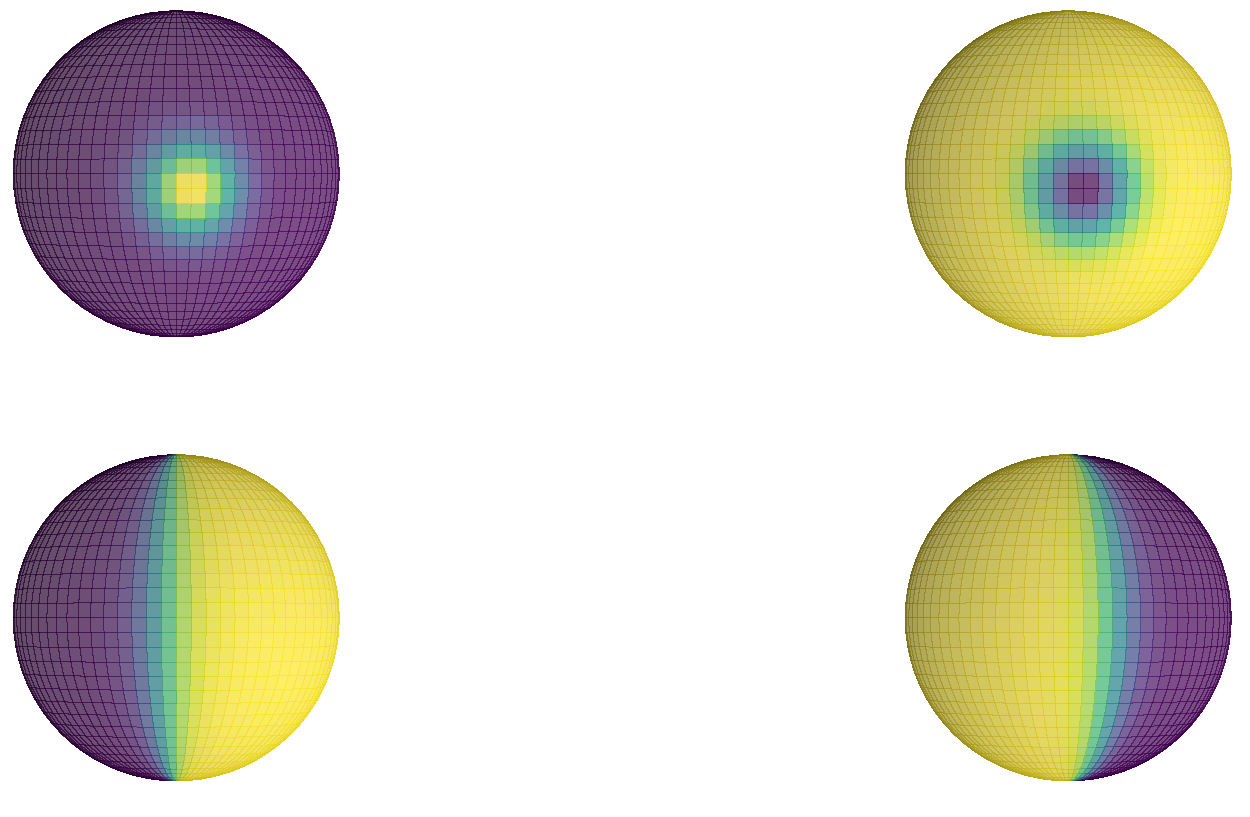
\includegraphics[scale=0.7,keepaspectratio]{fig/filters.png}};
			\node at (0.0,2.6) [color=black] {\small \textbf{Pre-selection filters}};
			\node at (-2.6,0.1) [color=black] {\scriptsize Point excitation};
			\node at (2.6,0.1) [color=black] {\scriptsize Point inhibition};
			\node at (-2.7,-2.4) [color=black] {\scriptsize Right-side excitation};
			\node at (2.7,-2.4) [color=black] {\scriptsize left-side excitation};
			
			\end{tikzpicture}
			\caption{Filters functions affecting the pre-selection phase.}
			\label{fig:filters}
		\end{center}
	\end{figure}
	
	
	\section{METHODOLOGY}
	\label{sec:methodology}

	\section{RESULTS}
	\label{sec:results}

	\section{CONCLUSIONS}
	\label{sec:conclusions}
	
	
	\addtolength{\textheight}{-12cm}   % This command serves to balance the column lengths
	% on the last page of the document manually. It shortens
	% the textheight of the last page by a suitable amount.
	% This command does not take effect until the next page
	% so it should come on the page before the last. Make
	% sure that you do not shorten the textheight too much.
	
	%%%%%%%%%%%%%%%%%%%%%%%%%%%%%%%%%%%%%%%%%%%%%%%%%%%%%%%%%%%%%%%%%%%%%%%%%%%%%%%%
	
	
	
	%%%%%%%%%%%%%%%%%%%%%%%%%%%%%%%%%%%%%%%%%%%%%%%%%%%%%%%%%%%%%%%%%%%%%%%%%%%%%%%%
	
	
	
	%%%%%%%%%%%%%%%%%%%%%%%%%%%%%%%%%%%%%%%%%%%%%%%%%%%%%%%%%%%%%%%%%%%%%%%%%%%%%%%%
	%\section*{APPENDIX}
	
	%Appendixes should appear before the acknowledgment.
	
	\section*{ACKNOWLEDGMENT}
	
	This research was only possible with the collaboration of colleagues from the robotics teams of both LAAS-CNRS (project ANITI) and LORIA-CNRS (project Creativ’Lab).
	
	
	
	%%%%%%%%%%%%%%%%%%%%%%%%%%%%%%%%%%%%%%%%%%%%%%%%%%%%%%%%%%%%%%%%%%%%%%%%%%%%%%%%
	
	
	\bibliographystyle{acm}
	\bibliography{references}	
	
	
	
\end{document}
